\section{RISC-V: A Compiler for a Modern RISC Architecture}

%\enquote{RISC-V is a recent, clean-slate, minimalist, and open ISA informed by mistakes of past ISAs. The goal of the RISC-V architects is for it to be effective for all computing devices, from the smallest to the fastest. Following von Neumann’s 70-year-old advice, this ISA emphasizes simplicity to keep costs low while having plenty of registers and transparent instruction speed to help compilers and assembly language programmers map actually important problems to appropriate, quick code.}\cite[p.~11]{Patterson2017}
% \begin{itemize}
% 	\item Introduced in 2011 X
% 	\item UC Berkely research project X
% 	\item Since then: rising in popularity X
% 	\item ISA = \enquote{instruction set architecture} X
% 	\item Was developed for: NO
% 	      \begin{itemize}
% 		      \item All sizes of processors: from embedded to high-performance computer
% 		      \item compatibility to popular software stacks and programming languages
% 		      \item serves as extendable base for customized accelerators
% 		      \item Should be stable
% 	      \end{itemize}
% 	\item One of the few ISAs which were developed this decade instead of the 1970s / 1980s X
% 	\item Open ISA: unlike most previous ISAs, it is free from a bond to a single comporation X
% 	\item Base ISA: \qVerb{RV321}.
% 	      Frozen, will never change, gives assembly programmers and compiler writers a stable target.
% 	\item The base instruction set is extendable using extensions like (multiply: \qVerb{RV32M}) or (double-precision floats: \qVerb{RV32D}).
% 	\item \enquote{RISC-V is a recent, clean-slate, minimalist, and open ISA informed by mistakes of past ISAs. The goal of the RISC-V architects is for it to be effective for all computing devices, from the smallest to the fastest. Following von Neumann’s 70-year-old advice, this ISA emphasizes simplicity to keep costs low while having plenty of registers and transparent instruction speed to help compilers and assembly language programmers map actually important problems to appropriate, quick code.}\cite[p.~11]{Patterson2017}
% \end{itemize} \cite[Chapter~1]{Patterson2017}.
%
% \TODO{Also interesting: \cite[p.~10]{Patterson2017}, \cite[Chapter~2]{Patterson2017}.}
%
% \begin{itemize}
% 	\item Present Some example instructions (Refer to chapter 3 of the RISC-V READER)
% 	\item Register layout \& count
% 	      RISC-V has 32 registers, ARM-32 16, x86\_32 has 8\\
% 	      Assembly includes all extensions\\
% 	      Concepts of \emph{pseudoinstructions}~\cite[p.~10]{Patterson2017}\\
% 	      Has basic instructions for add, sub, and logical operations\\
% 	      \emph{Check for all relationships between two registers, some conditional expressions involve rela- tionships between many pairs of registers. The compiler or assembly language programmer could use slt and the logical instructions and, or, xor to resolve more elaborate conditional expressions. The two remaining integer computation instructions Figure 2.1 help with assembly and}
% 	      r0 → constant 0 register\\
% 	      ~\cite[p.~18]{Patterson2017}
% 	\item ASM directives: \cite[p.~39]{Patterson2017}
% 	\item ASM includes 60 pseudoinstructions: \cite[p.~42]{Patterson2017}
% 	\item Another 32 Float registers, float load / store instructions: \cite[pp.~48f.]{Patterson2017}
% 	\item Refer to stack figure: \cite[p.~40]{Patterson2017}
% 	\item Calling convention
% \end{itemize}

\newpage

The \emph{RISC-V} \emph{ISA}\footnote{Short for: \enquote{instruction set architecture}} is a new and modern \emph{reduced instruction set} architecture focussed on simplicity and extendability.
It was originally developed at \emph{UC Berkely} in the context of a research project.
Since its initial introduction in 2011, the architecture has been rapidly growing in popularity.
During that time, it was managed and led by the \emph{RISC-V foundation}, consisting of many individuals contributing to the project.
Today, the corporate members of the RISC-V foundation include companies like \emph{Google}, \emph{Microsoft}, \emph{Samsung}, and \emph{IBM}.
Therefore, the popularity and commercial attractively of the technology is apparent.
However, unlike most previous ISAs, the RISC-V architecture is a completely open-source project and therefore not controlled by a single large corporate entity.
Unlike most of the previous ISAs which were developed during the 1970s or 80s, RISC-V is one of the few ISAs which were developed this decade.

\subsection{Register Layout}

\subsection{Memory Access Through the Stack}

\begin{figure}[h]
	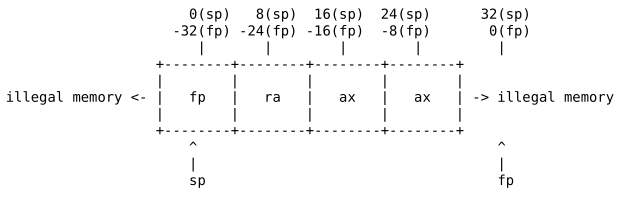
\includegraphics[width=\textwidth]{./riscv_stack_draft.png}
	\caption{\textcolor{red}{DRAFT:} Stack Memory on the RISC-V architecture}\label{fig:riscv_stack}
\end{figure}

\begin{itemize}
	\item In the current implementation, \qVerb{sp} includes legal memory locations
	\item \qVerb{fp} points to the first address after the last legal one
\end{itemize}

\subsection{Calling Convention}

\subsection{RISC-V Assembly}

\noindent
\begin{figure}[h]
	\begin{minipage}{.4\textwidth}
		\Lirsting[fancyvrb={frame=none}]{listings/riscv_simple.rush}
	\end{minipage}%
	\begin{minipage}{.6\textwidth}
		\Lirsting[raw=true, ranges={1-31,53-56}, fancyvrb={frame=none}]{listings/generated/riscv_simple.s}
	\end{minipage}
	\caption{Rush Program Alongside its RISC-V Output}\label{fig:rush_riscv_split}
\end{figure}

The rush program on the left side of Figure~\ref{fig:rush_riscv_split} shows a program which exists.
Because the assembler code of the \qVerb{foo} function would take up too much space in the assembler program, it is intentionally omitted from this listing.
Since the excluded function does not introduce any new concepts anyway, omitting it will not lead to a loss of explained content.
In line 1 of the rush program, a mutable global variable named \qVerb{m} is defined using the initial value 42.
In the main-function, \qVerb{m} is incremented by 1.
Next, the \qVerb{foo} function is called using m as its call argument.
In line 6, a return-statement is used to terminate the main-function explicitly.
However, the \qVerb{foo} function only calls the exit function on its own.
Therefore, the exit code of the program will be 43.

In line 1, the \qVerb{.global} assembler directive is used to declare the global symbol \qVerb{_start}~\cite[p~.36]{Patterson2017}.
On most architectures, the \qVerb{_start} label indicates the program's entry point, therefore marking the first instruction to be executed~\cite[p.~19]{Zhirkov2017-wk}
Object files using the ELF format are usually partitioned into several sections.
Here, every individual section exists to serve a special purpose.
For instance, the \qVerb{.text} section stores all CPU instructions to be executed.
Furthermore, the \qVerb{.data} and \qVerb{.rodata} sections store mutable and read-only data respectively~\cite[p.~76]{Zhirkov2017-wk}.
In line 5, the \qVerb{_start} label is defined using its name followed by a colon.
One might realize that the concepts of labels in RISC-V assembly can be compared to the labels and basic blocks introduced in the chapter about LLVM.
However, these labels do not come with all the constraints which were introduced by LLVM basic blocks.
Therefore, a label in assembly might even contain no instructions, does not have to be terminated and could even be terminated twice.
Here, terminating instructions mean jump- and return-instructions.
In line 6, the \qVerb{call} instruction is used to call the \qVerb{main..main} function.
This pseudoinstruction will jump to the first instruction of the specified target label whilst saving the address of the next instruction after the \qVerb{call} instruction in the register \qVerb{ra}.
Since this register holds the address of the next instruction after the function call, similarities to the call-stack of the rush VM can be noticed~\cite[p.~22]{Patterson2017}.
What strikes the eye here is that the already familiar \qVerb{main} contains the \qVerb{main..} prefix.
Due to name mangling implemented by this rush compiler, every function declared in a rush program will contain this prefix.
However, unlike function calls in LLVM, this call instruction must be used alongside the previously explained low-level calling conventions of RISC-V.

In the next line, the \qVerb{li} instruction is used to move the constant integer 0 into the register \qVerb{a0}~\cite[reference]{Patterson2017}.
In line 8, the \qVerb{exit} function is called, however, one cannot see the definition of this function inside the current file.
Since the exit-function is defined in a separate file, this scenario presents referencing an external library which is later resolved by the linker.
The instructions in the lines 7-8 are responsible for terminating the program using exit code 0.
These two instructions are always inserted at the end of the \qVerb{_start} label in order to terminate the program appropriately in case the rush code does not call \qVerb{exit} on its own.

Due to the function call in line 6, we will now shift our focus on the \qVerb{main..main} label in line 10.
An interesting observation is that labels can be called as if they were functions.
However, the \qVerb{call} instruction is only a pseudoinstruction which jumps to the target label whilst performing additional work during the process.
In line 11, the first line of the \qVerb{main} function, a comment indicates the beginning of the function's prologue.
In the rush compiler's implementation, each function contains a \emph{prologue} and an \emph{epilogue}.
The prologue is responsible for allocating space on the stack by incrementing \emph{sp} and \emph{fp} according to the amount of memory required in its function.

For instance, the \qVerb{addi} instruction in line 12 is used to decrement the value of the \qVerb{sp} register by 16.
However, an addition instruction is used even though subtraction is required.
In RISC-V, the \qVerb{addi} instruction requires one register and one immediate value as its operands.
The latter is the cause for the trailing \qVerb{i} (\emph{immediate}) in the instruction's name.
Since this immediate value can be negative, an additional instruction for immediate subtraction is redundant~\cite[reference]{Patterson2017}.
This example shows how the ISA omits redundant instructions were feasible.
In this case, the stack pointer is decremented by 16 since two 8-byte values are stored on the stack in the lines 13 and 14.
Here, the values of the registers for the frame pointer and the \emph{return address} (\emph{ra}) are saved on the stack.
This way, their values can be restored later before returning from this function.
In line 15, the frame pointer is adjusted according to the modifications made to the stack pointer.
The comment in the next line indicates the end of the prologue.
In short, the prologue performs important initialization before any other code of the newly called function is executed.

The comment in line 17 indicates the start of the function's body.
First, the previously explained \qVerb{li} instruction in line 18 places a constant 1 in register \qVerb{a0}.
Next, the \qVerb{ld} instruction in line 19 is used in order to load the value of the global variable \qVerb{m} into the register \qVerb{a0}~\cite[reference]{Patterson2017}.
Global variables, like \qVerb{m} in this example are saved under the \qVerb{.rodata}. section or under the \qVerb{.data} section if they are mutable.
In this example, \qVerb{m} is not declared as mutable and therefore saved under the \qVerb{.rodata} section.
The start of the \qVerb{.rodata} section is represented by the \qVerb{.section} assembler directive found in line 53.
Here, a label called \qVerb{m} is defined.
In this label, the \qVerb{.dword} directive is used to define the global initializer value of the variable.
In RISC-V, this directive stores 64 bit of information in successive memory doublewords~\cite[p.~39]{Patterson2017}.
The initializer value of the global variable is $42_{10}$ and represented as $\text{0x2a}_{16}$ in the assembly code. \TODO{Is specification of the base correct here?}
Since these data labels require their data to be specified in hexadecimal, the trailing comment shows the base 10, human-readable version of the number.
Because global variable are not saved on the stack, special instructions like \qVerb{ld} are required to interact with global variables stored in the program's data sections.

Now, the register \qVerb{a0} would contain 1 and \qVerb{a1} would contain 42.
In line 20, the \qVerb{add} instruction is used in order to save the sum of \qVerb{a0} and \qVerb{a1} in the register \qVerb{a2}.
Now, the value of \qVerb{a2} would be 43.
Next, the \qVerb{sd} instruction in line 21, saves the value of the register \qVerb{a2} at the memory location of the global variable \qVerb{m}, meaning that m is updated to reflect its new value 43.
It now becomes apparent that these instructions are responsible for the add-assign expression in line 4 of the rush program.
Another interesting observation is that the \qVerb{sd} instruction uses the temporary register \qVerb{t6} for saving temporary data~\cite[reference]{Patterson2017}.

Next, the previously explained \qVerb{ld} instruction in line 22 is used in order to load the value of the global variable into the register \qVerb{a0}.
Then, the \qVerb{call} instruction in line 23 is used in order to call the \qVerb{foo} function using the value of m as its argument.
However, one cannot easily observe how call arguments are passed here.
Like explained previously, the first integer argument of a function call must be placed in the register \qVerb{a0}.
Since \qVerb{m} was loaded into \qVerb{a0} previously, it is used as the call argument for \qVerb{foo} automatically.
Therefore, the \qVerb{foo} function would be called using 43 as its argument value.

Since the \qVerb{foo} instruction only calls the \qVerb{exit} function, its explanation will not be beneficial through the introduction of new concepts.
The final instruction of the main-function's body is the \qVerb{j} instruction in line 24.
This instruction will cause the CPU to jump to the address of the specified label.
In this example, the CPU will jump to the first instruction of the \qVerb{epilogue_0} label~\cite[p.~17]{Patterson2017}.
Therefore, the rush compiler uses the \qVerb{call} instruction for jumps caused by function calls and the \qVerb{j} instruction for jumps between blocks of the current function.

Like previously hinted, every function has a \emph{prologue} and an \emph{epilogue}.
Just like the name suggests, the epilogue is used to free any resources allocated by the function's prologue.
For instance, the frame pointer is restored to its state before the function call.
Furthermore, the epilogue restores the value saved in the \qVerb{ra} register in order to restore the return address.
Since the return address is vital for returning to the next instruction after the function call in the caller function, it is restored here so that this function returns control to the correct caller instruction.
Since the return address of the caller function is saved in the prologue, nested function calls will cause no issues.
If the prologue would not save the return address on the stack, a nested function call would overwrite the return address of the parent function, therefore creating a bug~\cite[p.33]{Patterson2017}.
Again, this design contains a lot of similarities to the call-design of the rush VM\@.
In the VM, the process of saving and restoring the return address was managed automatically by the VM\@.
However, here, the programmer has to manually pay attention to saving and restoring this important piece of data.
Therefore, implementing a call stack is definitely more demanding in RISC-V assembly than in the rush VM\@.
In line 30, the stack pointer is incremented again in order to deallocate memory used by the function.
Finally, the \qVerb{ret} instruction in line 31 is used in order to jump back to the instruction whose address is specified in the \qVerb{ra} register~\cite[reference]{Patterson2017}.

\subsection{The Core Library}

\subsection{The rush Compiler Targeting RISC-V Assembly}

